\chapter{Creating an architecture}

This chapter will view what goes into choosing a software architecture. What should you consider when choosing one and why.

\section{What is software architecture}
\label{sec:WhatIsSoftwareArchitecture}

A software architecture is:

\largequote{Software architecture is the process of converting software characteristics such as flexibility, scalability, feasibility, reusability, and security into a structured solution that meets the technical and the business expectations. \cite{softwareArchitectureDefinition}}

\section{Priorities}

As mentioned in the definition of software architecture \fullref{sec:WhatIsSoftwareArchitecture} a software architecture looks at the characteristics as flexibility, scalability, ect. These characteristics and their sub characteristics are defined by ISO 25010 \cite{iso25010}.

It is important to state the order in which EFFE values these quality attributes. Every decision will be based on this order and will be rationalized by this order.

What is EFFE looking for in an architecture? As mentioned in \fullref{sec:Intention} the first point points out the modularity and the interchangeability of these building blocks. The \textbf{maintainability} quality attribute has reusability and modularity as its sub characteristic. Thus is this the first focus of the software architecture.

The second focus is \textbf{compatability}. Compatibility is the degree to which a product, system or component can exchange information with other products, systems or components, and/or perform its required functions, while sharing the same hardware or software environment \cite{iso25010}. The system can be very modular but if the different functionalities cannot talk with each other you get nothing from the modularity.

As mentioned in first and second point the functionality may be shared between building blocks or not but each building block should be able to be functionality loose from the other building blocks. This is why \textbf{functional sustainability} will be the third focus.

With such a loosely coupled system one issue remains. The \textbf{security}. Because every functionality is loosely coupled it means that the functionalities will talk with each other over an open network or a closed network. If they talk on an open network the security needs to be checked constantly. On a closed network measures need to be taken to keep the network closed. That is the reason on why security is our fourth focus.

After running through these four quality attributes we have an application that can function without being overtaken by unintentional users. But in order to keep the intentional users satisfied the services or functions need to be reliable. Thus \textbf{reliability} will be our fifth focus.

When something is reliable it does not mean it is workable. Because if the site is not responding as fast as possible the user will get irritated and maybe leave the site. A study in 2018 of Google showed that the bounce rate between 3 second load time and 5 second load time is 58\% \cite{bounceRateDifference}. Thus in order for our users to be actually able to use the application in a responsive manner \textbf{performance efficiency} becomes our sixth focus.

There are only two quality attributes left. Portability and usability. Normally there is a good argument about why usability would be higher in the rankings. But because this research more focussed on the architecture of the application and not UX or UI \textbf{portability} will be our seventh focus and \textbf{usability} our eighth.

\subsection{Recap}
\label{sec:IsoRecap}

\begin{enumerate}
        \item maintainability
        \item Compatibility
        \item Functional sustainability
        \item Security
        \item Reliability
        \item Performance
        \item Portability
        \item Usability
\end{enumerate}

\section{What goes into choosing or creating an architecture}

\subsection{Creating an architecture}

So compared to choosing an architecture, creating one is something entirely different. An architecture does not exactly have a creator. This is because an architecture is just blueprint on how to create the software design. This is why the choice was made to interview current software architects and ask them the questions on how they made those choices.

This image was used to show how this research looks at architecture:

\begin{figure}[H]
	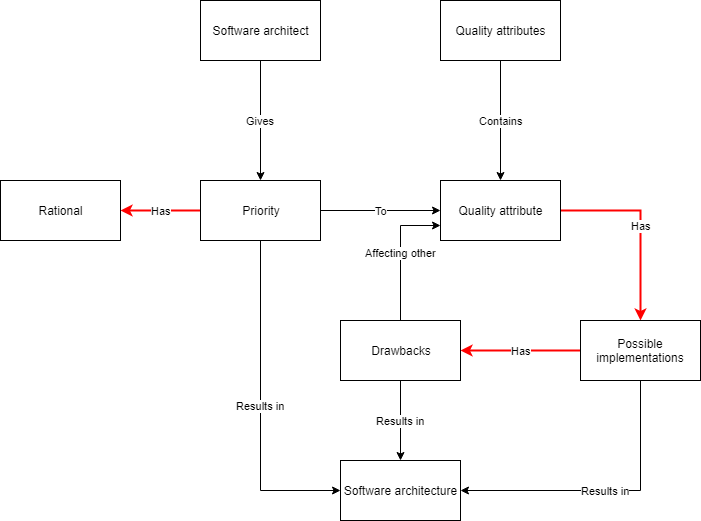
\includegraphics[width=\linewidth]{creating_architecture.png}
	\caption{How a software architecture is chosen}
\end{figure}
